\documentclass[a4paper,12pt]{article}
\usepackage{fullpage}
\usepackage{graphicx}
\usepackage{caption}
\usepackage{float}
\usepackage{hyperref}

\hypersetup{
    colorlinks,
    citecolor=blue,
    filecolor=black,
    linkcolor=blue,
    urlcolor=blue
}
\begin{document}
%\selectlanguage{english}
\pagenumbering{Roman}



\title{\begin{Huge}
\textbf{Simulation Tool for Smart Fridge and Sudoku Solver}
\end{Huge}}
\author{\begin{Large}
Sreenivas, Jonas and Mariusz
\end{Large}}
\date{\today}
\maketitle
\thispagestyle{empty}
\begin{center}
\begin{large}
\textbf{Software Design Document}
\end{large}
\end{center}
\newpage
\tableofcontents \newpage
\pagenumbering{arabic}
\section{Introduction}
\subsection{Purpose}
This document is a software design document , which describes the architecture and system design of the simulation tool for SmartFridge and Sudoku Solver. It is intended for developers of other projects and users who wish to you use the simulation tool.
\subsection{Scope}
\begin{itemize}
\item Create a large dataset of rendered images with groundtruth for SmartFridge and Sudoku solver which will be used by the respective projects.
\item This dataset can be used for classification or solving tasks with regards to the individual projects.
\item Provide a GUI to tune parameters of the simulation and an option to select or remove the rendered images.
\end{itemize}
\subsection{Overview}
The document describes about the system overview with its architecture, description of the data structures and data types used, component description (functionalities) and human interface design.

\newpage
\section{System Overview}
\subsection{Product Perspective}
It is a self contained project that can be used to simulate a large amount of data, which can potentially be used by developers, testers and users who wish to simulate images. These images include vegetables (in specific bananas and tomatoes) both in rotten and non-rotten form and sudoku puzzles with varying transformation and noise to evaluate other projects that require simulated data.

\subsection{Product Functions}
\begin{itemize}
\item User gives context for his application which we use in our simulation platform
\item The simulation platform generates a huge dataset of images with labels based on the context.
\end{itemize}
\subsection{Background Information}
The two teams: SmartFridge and Sudoku Solver require data which might be hard to collect. Thus, a simulation tool that renders images with ground truths can provide a large dataset that represents real images.
\section{System Architecture}
\begin{figure}[H]
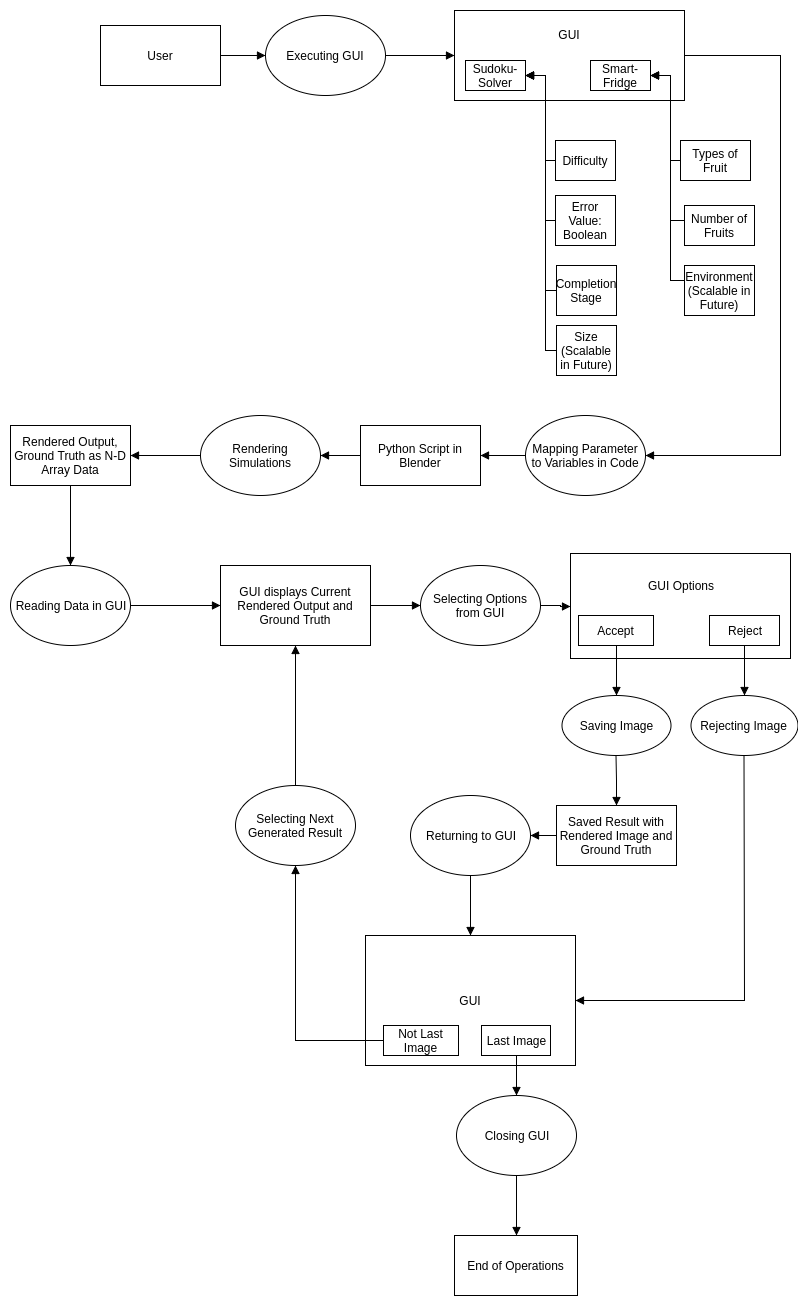
\includegraphics[scale=0.5]{system_workflow.png}
\caption{System Workflow}
\end{figure}
The individual modules at the top layer include the choice between SmartFridge and Sudoku solver. Once the choice is made, the user gives specific inputs with regards to his project. As an example, this includes the type of fruit in the case of SmartFridge. The next layer of choices include parameters for the rendering. For example, the mesh and material of the fruit. All these choices are used in the python script used by blender to generate rendered images.


\section{Data Design}
\subsection{Data Description}
For the user, the data choices are given in the user interface. In the internal code, these data choices are converted to float numbers and text which then is passed on to simulation tool (blender program) which decides what and how to render the images.
\subsection{Data Dictionary}
\begin{itemize}
\item Choice between Sudoku solver or SmartFridge: String of maximum size 20 characters.
\item Image Resolution: Integer type.
\item Parameter choices: Float numbers or string
\begin{itemize}
\item SmartFridge: String which describes the required fruits to render.
\item Sudoku Solver: Float numbers to render various difficulty choices.
\end{itemize}
\end{itemize}
\section{Component Design}
\begin{itemize}
\item  The GUI component provides choices between the two projects (SmartFridge and Sudoku solver). Based on the project choice, respective parameter choices are then shown to generate required rendered images. In the case of SmartFridge this corresponds to mesh and material. Also, in the GUI, image resolution can be changed by the user.
\item Sudoku solver component: We generate various difficulty sudoku puzzles with varying image transformations which includes deformations, angles and blur.
\item SmartFridge component: The type of fruit is decided based on the choice made in the GUI. Amount of fruits is also given as parameter with percentage of rotten vs non-rotten images.
\begin{itemize}
\item Mesh component: Based on the fruit choice and amount of rotten factor, the mesh is deformed accordingly based on user inputs.
\item Material component: Based on the fruit choice and amount of rotten factor, the material varies within the fruit based on user inputs.
\end{itemize}
\end{itemize}
\section{Human Interface Design}
\begin{figure}[H]
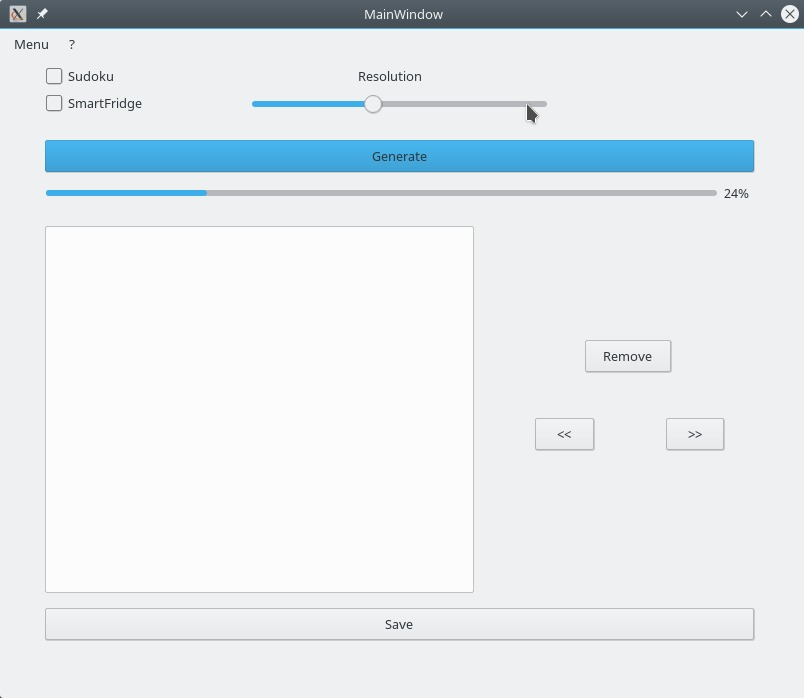
\includegraphics[scale=0.50]{UI.jpeg}
\caption{GUI design in the current state}
\end{figure}
\end{document}
